% One product search, step by step (phase 1).
% Build: tectonic --outdir . fig-search-flow-v1.tex
\documentclass[border=16pt]{standalone}
\usepackage[T1]{fontenc}
\usepackage[utf8]{inputenc}
\usepackage{helvet}
\renewcommand{\familydefault}{\sfdefault}
\usepackage{tikz}
\usetikzlibrary{arrows.meta,calc}

\definecolor{ink}{HTML}{0F2A33}
\definecolor{muted}{HTML}{5E7078}
\definecolor{line}{HTML}{C3CED2}
\definecolor{blue}{HTML}{1F5FA8}
\definecolor{orange}{HTML}{E2551F}
\definecolor{hubfill}{HTML}{EDF2F4}

\begin{document}
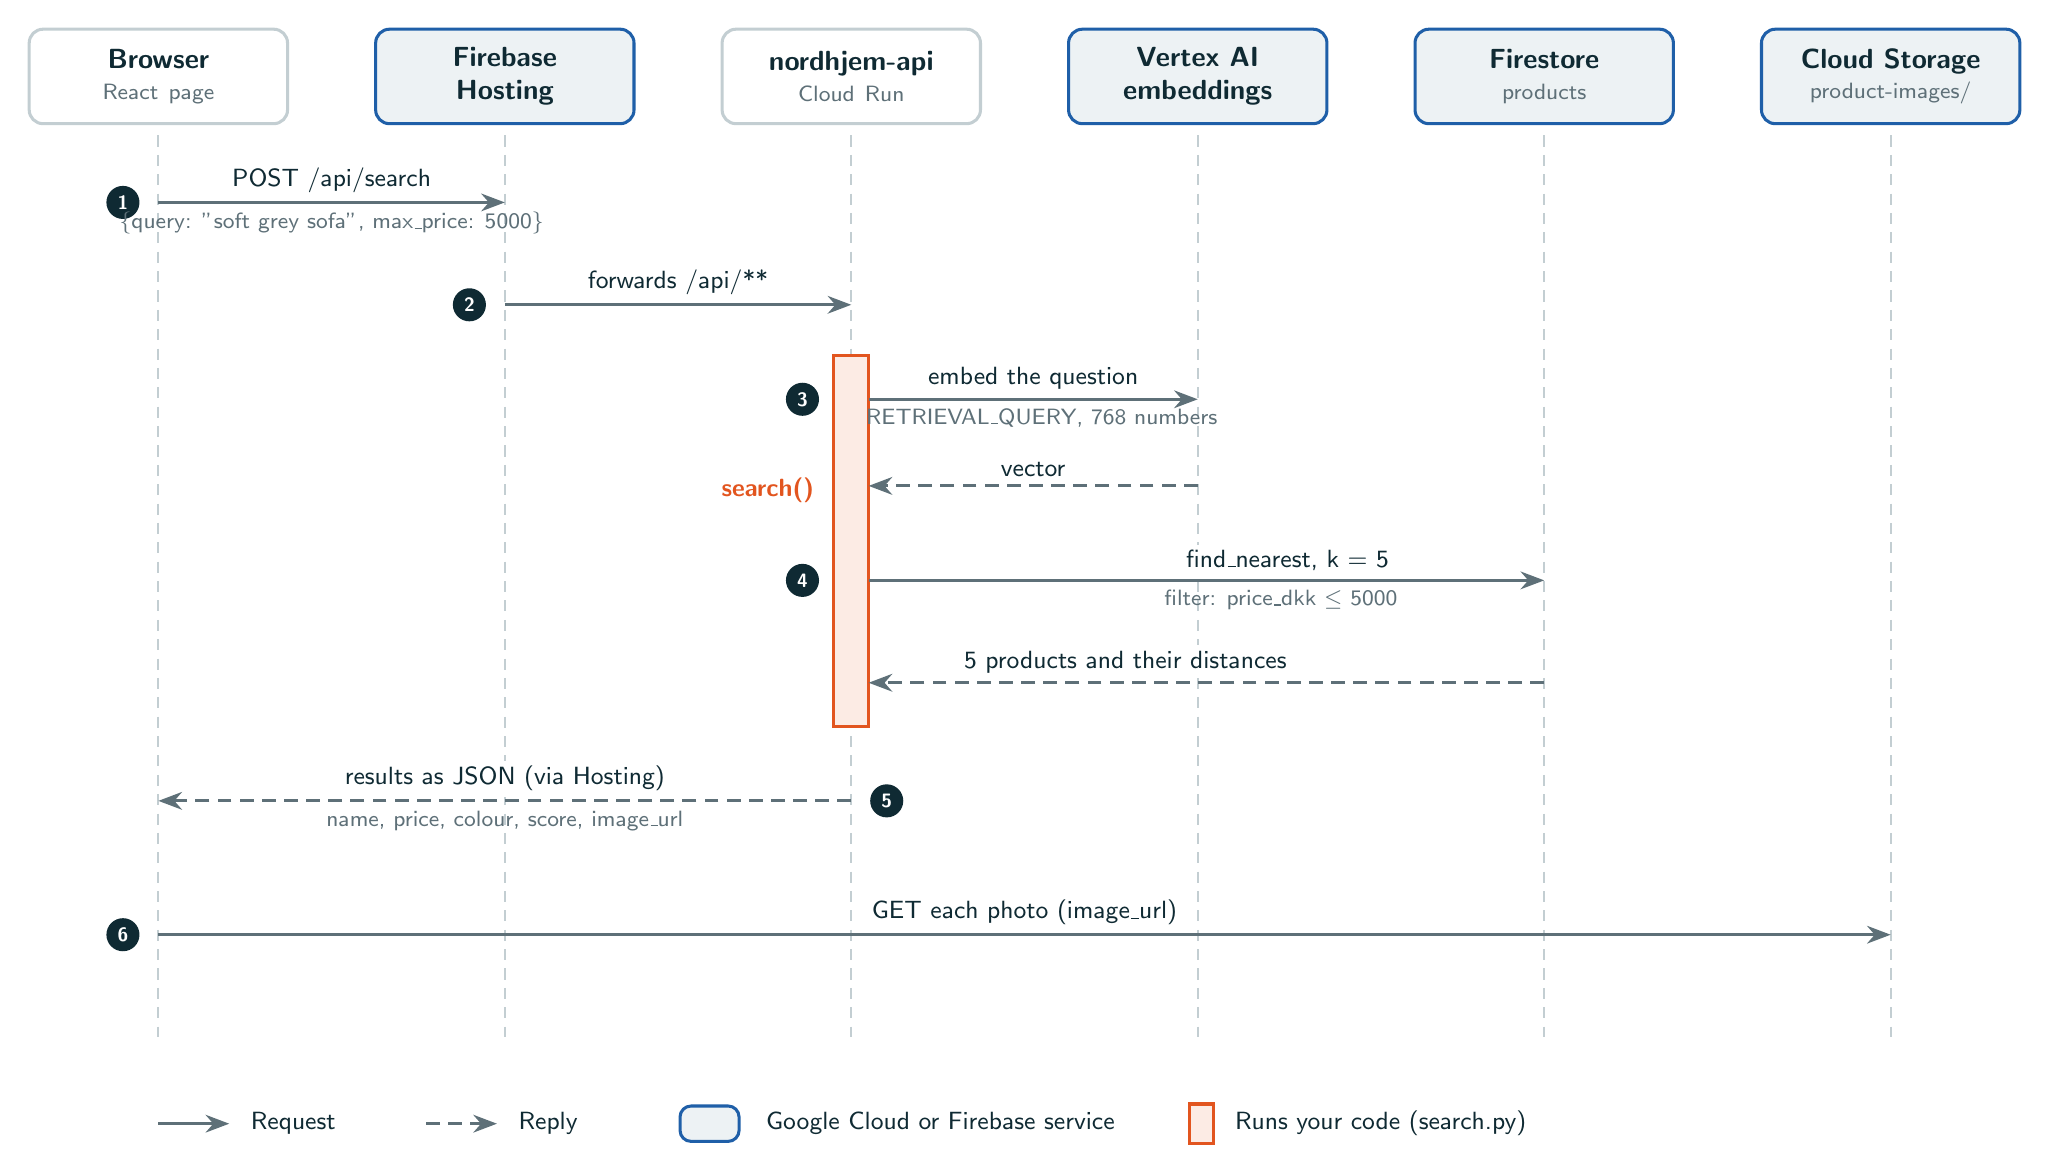
\begin{tikzpicture}[
  font=\sffamily,
  head/.style={rounded corners=5pt, draw=line, line width=1.1pt, fill=white,
    text=ink, align=center, text width=3.0cm, minimum height=1.2cm,
    inner sep=4pt, font=\sffamily\bfseries},
  gcp/.style={head, draw=blue, fill=hubfill},
  life/.style={line width=0.8pt, draw=line, dashed,
    dash pattern=on 4pt off 3pt},
  call/.style={line width=1.1pt, draw=muted, -{Stealth[length=3mm]}},
  back/.style={line width=1.1pt, draw=muted, dashed,
    dash pattern=on 5pt off 3pt, -{Stealth[length=3mm]}},
  msg/.style={text=ink, font=\small, fill=white, inner sep=2pt},
  num/.style={circle, fill=ink, text=white, font=\scriptsize\bfseries,
    inner sep=1.2pt, minimum size=0.42cm},
]

% x positions of the lifelines
\def\xb{0}     % browser
\def\xh{4.4}   % hosting
\def\xa{8.8}   % api
\def\xe{13.2}  % embeddings
\def\xf{17.6}  % firestore
\def\xs{22.0}  % storage
\def\ybot{-12.2}

\node[head] (b) at (\xb,0) {Browser\\[-1pt]{\footnotesize\mdseries\color{muted}React page}};
\node[gcp]  (h) at (\xh,0) {Firebase\\Hosting};
\node[head] (a) at (\xa,0) {nordhjem-api\\[-1pt]{\footnotesize\mdseries\color{muted}Cloud Run}};
\node[gcp]  (e) at (\xe,0) {Vertex AI\\embeddings};
\node[gcp]  (f) at (\xf,0) {Firestore\\[-1pt]{\footnotesize\mdseries\color{muted}products}};
\node[gcp]  (s) at (\xs,0) {Cloud Storage\\[-1pt]{\footnotesize\mdseries\color{muted}product-images/}};

\foreach \x in {\xb,\xh,\xa,\xe,\xf,\xs}
  \draw[life] (\x,-0.75) -- (\x,\ybot);

% search() runs on the api lifeline: written by you
\fill[orange!12] (\xa-0.22,-3.55) rectangle (\xa+0.22,-8.25);
\draw[orange, line width=1.1pt] (\xa-0.22,-3.55) rectangle (\xa+0.22,-8.25);
\node[text=orange, font=\small\bfseries, anchor=east] at (\xa-0.35,-5.25)
  {search()};

% 1. browser to hosting
\draw[call] (\xb,-1.6) -- node[msg, above=1pt] {POST /api/search} (\xh,-1.6);
\node[num] at (\xb-0.45,-1.6) {1};
\node[text=muted, font=\footnotesize, anchor=north] at ($(\xb,-1.6)!0.5!(\xh,-1.6)$)
  {\{query: "soft grey sofa", max\_price: 5000\}};

% 2. hosting forwards
\draw[call] (\xh,-2.9) -- node[msg, above=1pt] {forwards /api/**} (\xa,-2.9);
\node[num] at (\xh-0.45,-2.9) {2};

% 3. embed the question
\draw[call] (\xa+0.22,-4.1) -- node[msg, above=1pt] {embed the question} (\xe,-4.1);
\node[num] at (\xa-0.62,-4.1) {3};
\node[text=muted, font=\footnotesize, anchor=north] at ($(\xa,-4.1)!0.55!(\xe,-4.1)$)
  {RETRIEVAL\_QUERY, 768 numbers};
\draw[back] (\xe,-5.2) -- node[msg, above=1pt] {vector} (\xa+0.22,-5.2);

% 4. vector search in firestore
\draw[call] (\xa+0.22,-6.4) -- node[msg, above=1pt, pos=0.62]
  {find\_nearest, k = 5} (\xf,-6.4);
\node[num] at (\xa-0.62,-6.4) {4};
\node[text=muted, font=\footnotesize, anchor=north] at ($(\xa,-6.4)!0.62!(\xf,-6.4)$)
  {filter: price\_dkk $\le$ 5000};
\draw[back] (\xf,-7.7) -- node[msg, above=1pt, pos=0.62]
  {5 products and their distances} (\xa+0.22,-7.7);

% 5. reply to the page
\draw[back] (\xa,-9.2) -- node[msg, above=1pt] {results as JSON (via Hosting)} (\xb,-9.2);
\node[num] at (\xa+0.45,-9.2) {5};
\node[text=muted, font=\footnotesize, anchor=north] at ($(\xa,-9.2)!0.5!(\xb,-9.2)$)
  {name, price, colour, score, image\_url};

% 6. photos straight from storage
\draw[call] (\xb,-10.9) -- node[msg, above=1pt, pos=0.5]
  {GET each photo (image\_url)} (\xs,-10.9);
\node[num] at (\xb-0.45,-10.9) {6};

% ---- Legend ----
\draw[call] (0,-13.3) -- (0.9,-13.3);
\node[anchor=west, text=ink, font=\small] at (1.05,-13.3) {Request};
\draw[back] (3.4,-13.3) -- (4.3,-13.3);
\node[anchor=west, text=ink, font=\small] at (4.45,-13.3) {Reply};
\node[rounded corners=4pt, draw=blue, line width=1.1pt, fill=hubfill,
      minimum width=0.75cm, minimum height=0.45cm] (k1) at (7.0,-13.3) {};
\node[anchor=west, text=ink, font=\small] at ([xshift=0.2cm]k1.east)
  {Google Cloud or Firebase service};
\fill[orange!12] (13.1,-13.55) rectangle (13.4,-13.05);
\draw[orange, line width=1.1pt] (13.1,-13.55) rectangle (13.4,-13.05);
\node[anchor=west, text=ink, font=\small] at (13.55,-13.3)
  {Runs your code (search.py)};

\end{tikzpicture}
\end{document}
